\documentclass[12pt]{article}
\usepackage{fullpage}
\usepackage{amsthm}
\usepackage{amsfonts,amsmath, amssymb,latexsym,mathrsfs}
\usepackage[margin=1.15in]{geometry}
\usepackage{enumitem}
\setlength{\parindent}{0pt}
\usepackage{tikz-cd}
\usepackage{fancyhdr}
\usepackage{multicol}




\theoremstyle{definition}
\newtheorem{thm}{Theorem}[section]

\newtheorem{prop}{Proposition}[section]


\theoremstyle{definition}
\newtheorem{definition}{Definition}[section]

\theoremstyle{remark}
\newtheorem*{remark}{Remark}

\theoremstyle{definition}
\newtheorem{example}{Example}[section]


\theoremstyle{definition}
\newtheorem{lem}{Lemma}[section]


\theoremstyle{definition}
\newtheorem{cor}{Corollary}[section]


\date{}
\title{Final Exam Summary (Everything, formula)}

\begin{document}
\maketitle
\section{Integral}
\section{Riemann Sums}
\begin{enumerate}
	\item$\int_a^bf(x)dx= \lim_{n\rightarrow \infty} \sum_{i=1}^n f(x_i)\Delta x\text{\bf (Limit of Right-hand sum RIGHT(n))}$

	\item$\int_a^bf(x)dx= \lim_{n\rightarrow \infty} \sum_{i=0}^{n-1} f(x_i)\Delta x\text{\bf (Limit of Left-hand sum LEFT(n))}$

	\item$\int_a^bf(x)dx\approx  \sum_{i=0}^{n-1} f(\frac{x_i+x_{i+1}}{2})\Delta x\text{\bf (Limit of Mid sum MID(n))}$

	\item$\int_a^bf(x)dx\approx \sum_{i=0}^{n-1} \frac{f(x_i)+f(x_{i+1})}{2}\Delta x\text{\bf (Limit of Trapezoid sum TRAP(n))}$

	\item$\Delta(x)=\dfrac{b-a}{n}$

	\item$\frac{LEFT(n)+RIGHT(n)}{2}=TRAP(n)$
	\item$MID(n)\neq TRAP(n)$

	\item Error estimation: $|LEFT(n) - f(x)|<|LEFT(n)-RIGHT(n)|=(f(b)-f(a))\Delta x$. This usually gives a bound for $n$.
\end{enumerate}



\subsection{Properties of Riemann sums:}
\begin{enumerate}
\item If the graph of $f$ is increasing on $[a,b]$, then $LEFT(n)\leq \int^b_a f(x) dx \leq RIGHT(n)$
\item If the graph of $f$ is decreasing on $[a,b]$, then $RIGHT(n)\leq \int^b_a f(x) dx \leq LEFT(n)$
\item If the graph of $f$ is concave up on $[a,b]$, then $MID(n)\leq \int^b_a f(x) dx \leq TRAP(n)$
\item If the graph of $f$ is concave down on $[a,b]$, then $TRAP(n)\leq \int^b_a f(x) dx \leq MID(n)$
\end{enumerate}
\subsection{Properties of Definite Integrals}	
	\begin{enumerate}
		\item $\int^a_b f(x) dx = -\int^b_a f(x) dx$
		\item $\int^a_b f(x) dx+\int^b_c f(x) dx=\int^a_c f(x) dx$
		\item $\int^a_b (f(x)\pm g(x)) dx=\int^a_b f(x) dx \pm \int^a_b g(x) dx$
		\item $\int^a_b cf(x) dx = c \int^a_b f(x) dx$
		\item Symmetry due to the oddity of the function.
		\item Average value of function $f(x)$ in $[a,b]$ is $\frac{1}{b-a} \int_{a}^{b}f(x)dx$.
	\end{enumerate}

\begin{thm}
\textbf{The Fundamental Theorem of Calculus}:

If $f$ is continuous on interval $[a,b]$ and $f(t)=F'(t)$, then $\int^b_a f(t) dt = F(b)-F(a).$
\textbf{Second FTC (Construction theorem for Antiderivatives)}
If $f$ is a continuous function on an interval, and if $a$ is any number in that interval then the function $F$ defined on the interval as follows is an antiderivative of $f$:

\[F(x)=\int^x_a f(t) dt\]
\end{thm}

\begin{enumerate}
\item	$\int C dx = 0$
\item	$\int kdx=kx+C$
\item	$\int x^ndx=\frac{x^{n+1}}{n+1}+C, (n \neq -1)$
\item	$\int \frac{1}{x}dx = \ln|x|+C$
\item	$\int e^xdx=e^x+C $
\item	$\int \cos xdx=\sin x + C $
\item	$\int \sin xdx=-\cos x + C $

\end{enumerate}


Properties of antiderivatives:

\begin{enumerate}
\item $\int (f(x) \pm g(x))dx=\int f(x) dx \pm \int g(x) dx$
\item $\int cf(x) dx = c \int f(x) dx$
\end{enumerate}




\subsection{Integration Techniques}
\begin{enumerate}
	\item Guess and Check
	\item Substitution $du=f(x)'dx$ if $u=f(x)$
	\item By parts $\int u dv=uv-\int v du$
	\item Partial fractions $\frac{p(x)}{(x+c_1)^2(x+c_2)(x^2+c_3)}=\frac{A}{x+c_1}+\frac{B}{(x+c_1)^2}+\frac{C}{x+c_2}+ \frac{Dx+E}{x^2+c_3}$
	\item Trig substitution:
	If the above method does not work and you have terms of $A\pm Bx^{2}$, then we will do trig substitution.\\
If you have terms of $A-Bx^{2}$, you should try substitute $x=\sqrt{\frac{A}{B}}\sin \theta$.\\
If you have terms of $A+Bx^{2}$, you should try substitute $x=\sqrt{\frac{A}{B}}\tan \theta$.\\
Using the relation, $\sin^{2}\theta+\cos^{2}\theta=1$ and $\tan^{2}\theta+1=\sec^{2}\theta$ to simplify.
\end{enumerate}


\section{Find Area/Volumes by slicing}

\begin{enumerate}
	\item Compute the area: Think about slicing the area into parallel line segments.
	\item Disk Method:\\
	Horizontal axis of revolution ($x$-axis): $V = \int_a^b \pi(f(x)^2 - g(x)^2)dx$\\
	Vertical axis of revolution ($y$-axis): $V = \int_a^b \pi(f(y)^2 - g(y)^2)dy$
	\item Shell Method:\\
	Horizontal axis of revolution ($x$-axis): $V = \int_a^b 2\pi y(f(y) - g(y))dy$\\
		Vertical axis of revolution ($y$-axis): $V = \int_a^b 2\pi x(f(x) - g(x))dx$

\end{enumerate}

\subsection{Mass}
The basic formula we are doing is:\begin{enumerate}
\item One dimensional: $M=\delta l$ where $M$ is the total mass, $\delta$ is the density, $l$ is line.
\item
Two dimensional: $M=\delta A$ where $M$ is the total mass, $\delta$ is the density, $A$ is Area.
\item Three dimensional (real world): $M=\delta V$ where $M$ is the total mass, $\delta$ is the density, $V$ is Volume.
\end{enumerate}



\subsection{Work}

Key formula we are using:\\
$\text{Work done = Force} \cdot \text{Distance}$ or 
$W=F\cdot s$

Integration version:
$W = \int^b_a F(x) dx$


\subsection{L'Hopital's rule}

L’Hopital’s rule: If $f$ and $g$ are differentiable and (below $a$ can be $\pm \infty$)\\
i)$f(a) = g(a) = 0$ for finite $a$, \\
Or ii)$\lim_{x\to a} f(x)=\lim_{x\to a} g(x)= \pm \infty$,\\ 
Or iii)$\lim_{x\to \infty} f(x)= \lim_{x\to \infty} g(x) = 0$
then 
\textcolor{red}{$\lim_{x\to a}\frac{f(x)}{g(x)} = \lim_{x\to a} \frac{f'(x)}{g'(x)} $}


\section{Improper integral}
There are two types of improper integral.

\begin{itemize}
	\item The first case is where we have the limit of the integration goes to infinity, i.e. $\lim_{b \to \infty} \int^b_a f(x) dx$.
	\item The integrand goes to infinity as $x \to a$.
\end{itemize}

\subsection{Converges or diverges?}

\begin{enumerate}
	\item Check by definition, this means check the limit directly.
	\item $p$-test.\\
	\includegraphics*[width=0.9\textwidth]{1.png}
	\item Exponential decay test. 
	\textcolor{red}{$\int^\infty_0 e^{-ax} dx$} converges for $a>0$.
	\item Comparison test.\\
	If $f(x)\geq g(x) \geq 0$ on the interval $[a,\infty]$ then,\begin{itemize}
	\item If $\int^\infty_a f(x) dx$ converges then so does $\int^\infty_a g(x) dx$.
	\item If $\int^\infty_a g(x) dx$ diverges then so does $\int^\infty_a f(x) dx$.
	\end{itemize}
	\item Limit Comparison theorem.\\
	Limit Comparison Test. If $f(x)$ and $g(x)$ are both positive  on the interval $[a,b)$ where $b$ could be a real number or infinity.
	and
	\textcolor{red}{$\lim_{x\to b}\frac{f(x)}{g(x)} = C$} such that $0 < C < \infty$
	then the improper integrals $\int^b_a f(x) dx$ and $\int^b_a g(x) dx$ are either both convergent or both divergent.

\end{enumerate}

\section{Probability}
\subsection{PDF and CDF}
\begin{definition}
A function $p(x)$ is a \textbf{probability density function} or PDF if it satisfies the following conditions
\textcolor{red}{\begin{itemize}
\item $p(x) \geq 0$ for all $x$.
\item $\int_{-\infty}^\infty p(x) = 1.$
\end{itemize}}
\end{definition}

\begin{definition}
A function $P(t)$ is a \textbf{Cumulative Distribution Function} or cdf, of a density function $p(t)$, is defined by 
$P(t) =\int_{-\infty}^t p(x) dx $,
which means that $P(t)$ is the antiderivative of $p(t)$ with the following properties:
\textcolor{red}{\begin{itemize}
\item $P(t)$ is increasing and $0\leq P(t)\leq 1$ for all $t$.
\item $\lim_{t \to \infty}P(t)=1.$
\item $\lim_{t \to -\infty}P(t)=0.$
\end{itemize}}
\end{definition}

Moreover, we have $\int_a^b p(x)dx=P(b)-P(a)$.

\subsection{Probability, mean and median}

\subsubsection*{Probability}
Let us denote $X$ to be the quantity of outcome that we care ($X$ is in fact, called the random variable).
$\mathbb{P}\{a\leq X\leq b\}=\int_a^b p(x)dx=P(b)-P(a)$\\
$\mathbb{P}\{X\leq t\}=\int_{-\infty}^t p(x)dx=P(t)$\\
$\mathbb{P}\{X\geq s\}=\int_{s}^\infty p(x)dx=1-P(s)$

\subsubsection*{The mean and median}
\begin{definition}
A \textbf{median} of a quantity $X$ is a value $T$ such that the probability of $X\leq T$ is $1/2$. Thus we have  $T$ is defined such that
$\int_{-\infty}^T p(x) dx=1/2$  or $P(T)=1/2$.
\end{definition}
\begin{definition} A \textbf{mean} of a quantity $X$ is the value given by
	\[ Mean= \frac{\text{Probability of all possible quantity}}{\text{Total probability}}= \frac{\int_{-\infty}^{\infty}xp(x)dx}{\int_{-\infty}^{\infty}p(x)dx}=\frac{\int_{-\infty}^{\infty}xp(x)dx}{1}=\int_{-\infty}^{\infty}xp(x)dx. \]
\end{definition}

\subsubsection*{Normal Distribution}
\begin{definition}
A normal distribution has a density function  
\textcolor{red}{$p(x)=\frac{1}{\sigma \sqrt{2 \pi}}e^{-\frac{(x-\mu)^2}{2\sigma^2}}$} where $\mu$ is the mean of the distribution and $\sigma$ is the standard deviation, with $\sigma > 0$.
The case $\mu = 0$, $\sigma = 1$ is called the standard normal distribution.

\end{definition}

\section{Sequences and Series}
\subsection{Sequence}

If a sequence $s_n$ is bounded and monotone, it converges.


\subsection{Series}

Convergence Properties of Series:
\begin{enumerate}
\item If $\sum_{n=1}^{\infty} a_n$ and $\sum_{n=1}^{\infty} b_n$ converge and if $k$ is a constant, then

$\sum_{n=1}^{\infty} (a_n+b_n)$ converges to$\sum_{n=1}^{\infty} a_n + \sum_{n=1}^{\infty} b_n$.\\
$\sum_{n=1}^{\infty} ka_n$ converges to $k\sum_{n=1}^{\infty} a_n$

\item Changing a finite number of terms in a series does not change convergence,
\item  If $\lim_{n \to \infty}a_n\neq 0$ or $\lim_{n \to \infty}a_n$ does not exist, then
$\sum_{n=1}^{\infty} a_n$ diverges. (\textbf{!})
\item If $\sum_{n=1}^{\infty} a_n$ diverges, then $\sum_{n=1}^{\infty} a_n$ diverges if $k\neq 0$.
\end{enumerate}
Moreover, there are several test to determine if a series is convergent.
\begin{enumerate}
\item \textbf{The Integral Test}\\
Suppose $a_n = f(n)$, where $f(x)$ is decreasing and positive.
\\a. If $\int_1^\infty f(x) dx$ converges, then $\sum_{n=1}^{\infty} a_n$ an converges.
\\b. If $\int_1^\infty f(x) dx$ diverges, then $\sum_{n=1}^{\infty} a_n$ an diverges.

\item \textbf{p-test}\\
The $p$-series $\sum_{n=1}^{\infty} 1/n^p$ converges if $p > 1$ and diverges if $p \leq 1$.

\item \textbf{Comparison Test}\\
Suppose $0 \leq a_n \leq b_n$ for all $n$ beyond a certain value.
\\ a. If $\sum_{n=1}^{\infty} b_n$ converges, then $\sum_{n=1}^{\infty} a_n$ converges.
\\ b. If $\sum_{n=1}^{\infty} a_n$ diverges, then $\sum_{n=1}^{\infty} b_n$ diverges.

\item \textbf{Limit Comparison Test}\\
Suppose $a_n > 0$ and $b_n > 0$ for all $n$. If
$\lim_{n\to \infty}a_n/b_n= c$ where $c > 0$,
then the two series $\sum_{n=1}^{\infty} a_n$ and $\sum_{n=1}^{\infty} b_n$ either both converge or both diverge.

\item \textbf{Convergence of Absolute Values Implies Convergence}\\
If $\sum_{n=1}^{\infty}|a_n|$ converges, then so does $\sum_{n=1}^{\infty} a_n$.

\item \textbf{The Ratio Test}
For a series $\sum_{n=1}^{\infty} a_n$, suppose the sequence of ratios $|a_{n+1}|/|a_n|$ has a limit:
$\lim_{n\to \infty}|a_{n+1}|/|a_n| = L$, then
\begin{itemize}
\item If $L < 1$, then $\sum_{n=1}^{\infty} a_n$ converges.
\item If $L > 1$, or if $L$ is infinite, then $\sum_{n=1}^{\infty} a_n$ diverges.
\item If $L = 1$, the test does not tell anything about convergence of $\sum_{n=1}^{\infty} a_n$ (!).
\end{itemize}

\item \textbf{Alternating Series Test}
A series of the form $\sum_{n=1}^{\infty} (-1)^{n-1}a_n = a_1 - a_2 + a_3 - a_4 + \ldots + (-1)^{n-1}a_n + \ldots$
converges if
$0 < a_{n+1} < a_n$ for all $n$ and $lim_{n \to \infty}a_n = 0$.

Error of alternating test: let $S = \lim_{n\to \infty}S_n$, then have $|S - S_n| < a_{n+1}$.
\end{enumerate}

Notably, We say that the series $\sum_{n=1}^{\infty} a_n$ is
\begin{itemize}
\item absolutely convergent if $\sum_{n=1}^{\infty} a_n$ and $\sum_{n=1}^{\infty}|a_n|$ both converge.
\item conditionally convergent if $\sum_{n=1}^{\infty} a_n$ converges but $\sum_{n=1}^{\infty}|a_n|$ diverges.
\end{itemize}
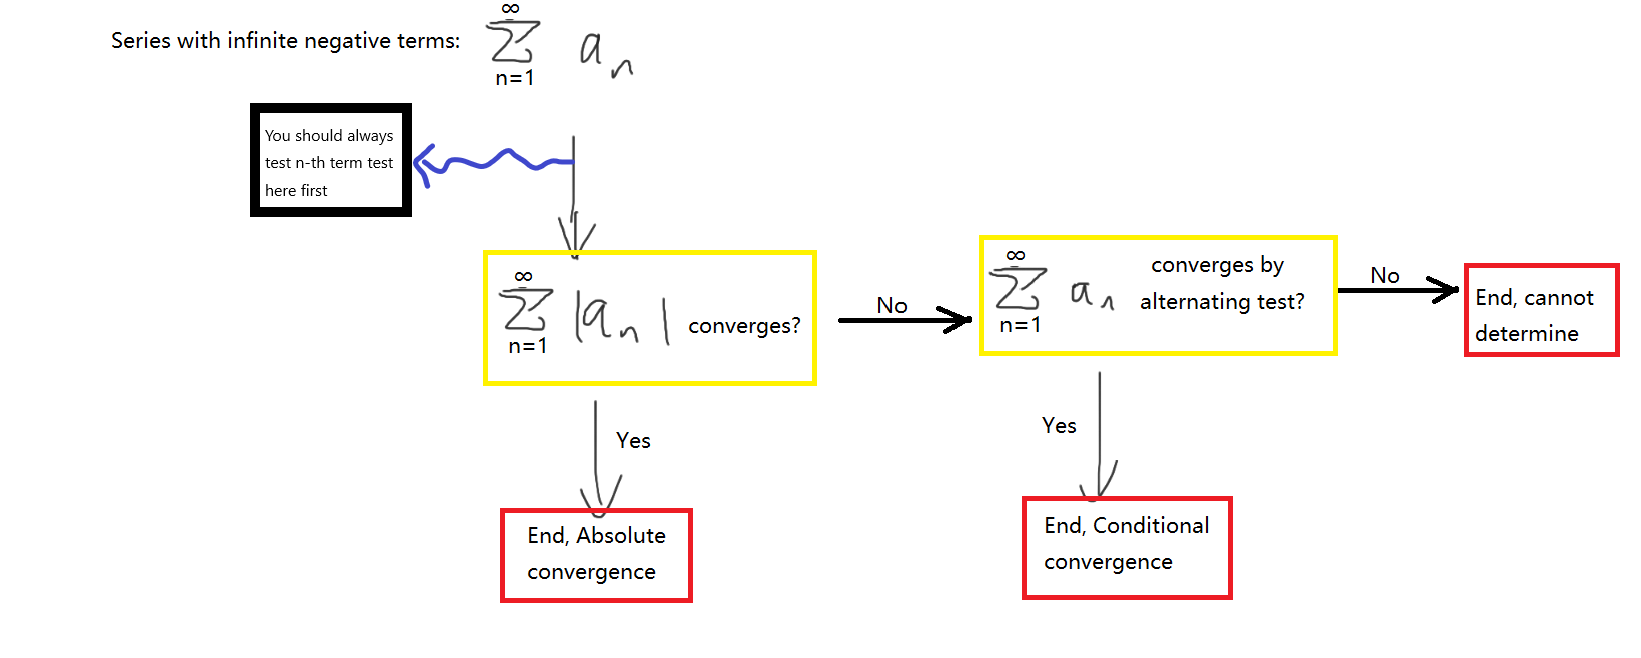
\includegraphics[width=1\textwidth]{program2.png}


\begin{multicols}{2}
Test we consider for proving convergence:
\begin{enumerate}
	\item The integral test
	\item p-test
	\item Comparison test
	\item Limit comparison test
	\item Check the absolute convergence of the series
	\item Ratio Test
	\item Alternating Series Test
\end{enumerate}
\columnbreak



Test we consider for proving divergence:
\begin{enumerate}
	\item The integral test
	\item p-test
	\item Comparison test
	\item Limit comparison test
	\item Ratio Test
	\item Check $\lim_{n \to \infty} \neq 0$ or $\lim_{n \to \infty}$ does not exist.
\end{enumerate}
\end{multicols}

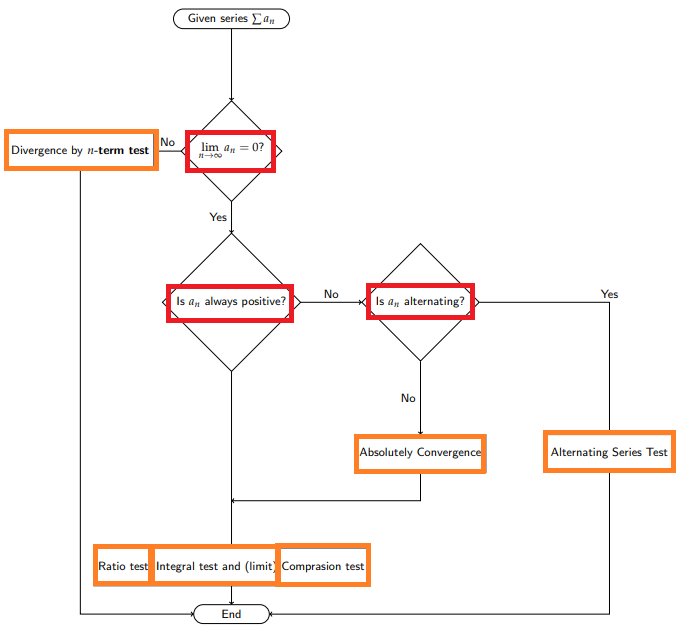
\includegraphics[width=1\textwidth]{program.png}


\subsection{Geometric Series}
There is a special series that we learn about, which is the Geometric Series, notice that the formula on the right hand side is what we called closed form. 
A finite geometric series has the form
\textcolor{red}{\[a + ax + ax^2 + \cdots + ax^{n−2} + ax^{n−1}=\frac{a(1-x^n)}{1-x}\text{ For } x \neq 1\]}
An infinite geometric series has the form
\textcolor{red}{\[a + ax + ax^2 + \cdots + ax^{n−2} + ax^{n−1}+ax^n +\cdots=\frac{a}{1-x}\text{ For } |x| < 1\]}

\newpage

\subsection{Power Series}
\begin{definition}
	A power series about $x = a$ is a sum of constants times powers of $(x - a)$: \\
	$C_0 + C_1(x - a) + C_2(x - a)^2 + \ldots + C_n(x - a)^n + \ldots =	\sum_{n
	=0}^{\infty}	C_n(x - a)^n$.
\end{definition}
Moreover, each power series falls into one of the three following cases, characterized by its radius of convergence, $R$.
\begin{itemize}
\item The series converges only for $x = a$; the radius of convergence is defined to be $R = 0$.
\item The series converges for all values of $x$; the radius of convergence is defined to be
$R = \infty$.
\item There is a positive number $R$, called the radius of convergence, such that the series
converges for $|x - a| < R$ and diverges for $|x - a| > R$. 
\end{itemize}
How to find radius of convergence: consider ratio test

The interval of convergence is the interval between $a - R$ and $a + R$, including any
endpoint where the series converges.

\subsection{Taylor Polynomial}
\textcolor{red}{Taylor Polynomial of Degree $n$ Approximating $f(x)$ for $x$ near $a$} is \[f(x) \approx P_n(x)
= f(a) + f'(a)(x-a) + \frac{f''(a)}{2!}(x-a)^2 + \frac{f'''(a)}{3!}(x-a)^3  + \ldots + \frac{f^{(n)}(a)}{n!} (x-a)^n\]
We call $P_n(x)$ the Taylor polynomial of degree $n$ centered at $x = a$, or the Taylor poly
nomial about $x =a$.
\subsection{Taylor Series}
\textcolor{red}{Taylor Series for $f(x)$ about $x=a$} is \[f(x) = f(a) + f'(a)(x-a) + \frac{f''(a)}{2!}(x-a)^2 + \frac{f'''(a)}{3!}(x-a)^3  + \ldots + \frac{f^{(n)}(a)}{n!} (x-a)^n+ \ldots \]
We call $P_n(x)$ the Taylor polynomial of degree $n$ centered at $x = a$, or the Taylor poly
nomial about $x =a$.

$f^{(n)}(a)= \{\text{coefficient of }x^n\}*n!$.

Moreover, there are \textcolor{red}{several important cases} that we consider, each of them is an Taylor expansion of a function about $x=0$:
\begin{itemize}
\item $e^{x}= 1 + x + \frac{x^2}{2!} + \frac{x^3}{3!} + \frac{x^4}{4!} + \frac{x^5}{5!} + \frac{x^6}{6!} + \frac{x^7}{7!} + \frac{x^8}{8!} + \cdots\text{ converges for all } x$
\item $\sin(x)=\sum\limits_{n=0}^\infty \dfrac{x^{2n+1}}{(2n+1)!}\cdot(-1)^n = x-\dfrac{x^3}{3!}+\dfrac{x^5}{5!}-\dfrac{x^7}{7!}+\dots\text{ converges for all } x$
\item $\cos(x)=\sum\limits_{n=0}^\infty \dfrac{x^{2n}}{(2n)!}\cdot(-1)^n = 1-\frac{x^2}{2!}+\frac{x^4}{4!}-\frac{x^6}{6!}+\dots \text{ converges for all } x$
\item $(1 + x)^p = \sum_{k=0}^{\infty} \binom{p}{k} x^k= \sum_{k=0}^{\infty} \frac{p!}{k!(p-k)!} x^k=1 + px + \frac{p(p - 1)}{2!}x^2 + \frac{p(p - 1)(p - 2)}{3!}x^3 + \cdots \text{ converges for } -1 < x < 1$.
\item $\ln(1+x) =\sum_{n = 0}^{\infty}\frac{(-1)^nx^{n+1}}{n+1}= x-\frac{x^2}{2}+\frac{x^3}{3}-\frac{x^4}{4}+\cdots,$

\end{itemize}
Moreover, we can definitely find Taylor Series based on the existing series using \textcolor{red}{four methods}:\\
Substitude/Differentiate/Integrate	/Multiply
	

\section{Parametric Equations and Polar Coordinate}
\subsection{Parametric Equations}

Summarize, we have the \textcolor{red}{slope}:$\frac{dy}{dx}=\frac{dy/dt}{dx/dt}$
and the \textcolor{red}{concavity} of the parametrized curve to be
$\frac{d^2y}{dx^2}=\frac{(dy/dx)/dt}{dx/dt}$

The quantity $v_x = dx/dt$ is the instantaneous velocity in the $x$-direction; $v_y = dy/dt$ is the
instantaneous velocity in the $y$-direction.
And we call that $(v_x,v_y)$ to be the velocity vector.

The \textcolor{red}{instantaneous speed} :$v = \sqrt{(dx/dt)^2 + (dy/dt)^2} =\sqrt{(v_x)^2 + (v_y)^2}$.\\


Moreover, the \textcolor{red}{distance} traveled from time $a$ to $b$ is $\int^b_a v(t) dt = \int_a^b \sqrt{(dx/dt)^2 + (dy/dt)^2} dt$

\subsection{Polar Coordinate}


\subsubsection{Relation between Cartesian and Polar}

\textcolor{red}{Cartesian to Polar}: $(x,y) \to (r= \sqrt{x^2 + y^2}, \theta) \text{ (Here we have that } \tan \theta = \frac{y}{x} \text{)}$
$\theta$ does not have to be $\arctan(\frac{y}{x})$!

Polar to Cartesian: $(r,\theta) \to (x=r \cos \theta, y=r \sin \theta)$

\subsubsection{Slope, Arc length and Area in Polar Coordinates}
\textcolor{red}{slope} of to be 
$\frac{dy}{dx}=\frac{dy/d\theta}{dx/d\theta}$

The \textcolor{red}{arc length} from angle $a$ to $b$ is $\int_a^b \sqrt{(dx/d\theta)^2 + (dy/d\theta)^2} d\theta=\int_a^b \sqrt{r^2 + (dr/d\theta)^2} d\theta$

Fact: \textcolor{red}{area of the sector} with angle $\theta$ is $1/2 r^2 \theta$, we have that for a curve $r = f(\theta)$, with \textcolor{red}{$f(\theta)$ continuously of the same sign}, the area of the region enclosed is $\frac{1}{2}\int^{b}_{a}f(\theta)^2 d\theta$.


\end{document} 